\pdfoutput=1 % only if pdf/png/jpg images are used
\documentclass[a4paper,10pt]{article}
%\documentclass[a4paper,10pt]{scrartcl}
%\documentclass[smallcondensed,referee]{svjour3}
\usepackage{geometry}
\geometry{a4paper,left=34mm,right=34mm, top=26mm, bottom=32mm}
%\geometry{a4paper}
\raggedbottom
\widowpenalty=10000
\clubpenalty=10000 
\usepackage{graphics}  
\usepackage{graphicx}
\usepackage{subfigure}
\usepackage{amsmath}
\usepackage[amssymb]{SIunits}
%\usepackage[load-configurations=abbreviations,tight-spacing=true,separate-uncertainty,bracket-numbers = false]{siunitx} % JINST cannnot handle siunitx !!
\usepackage{nicefrac}
\usepackage[english]{babel}
\usepackage{lineno}
\usepackage{epstopdf}
\usepackage{stfloats}
%\usepackage{upgreek}
\usepackage{verbatim}
\usepackage{url}
\usepackage{xcolor}
\usepackage{url}
%\usepackage{draftwatermark}
%\SetWatermarkScale{5}
\usepackage{setspace}


%general stuff 
\newcommand{\e}{\ensuremath{\mathnormal{e}}}
\newcommand{\h}{\ensuremath{\mathnormal{h}}}
\newcommand{\eV}{\ensuremath{\mathnormal{eV}}}
\newcommand{\cspeed}{\ensuremath{\mathnormal{c}}}

%tscope specific
\newcommand{\DESY}{\ensuremath{\textrm{DESY}}}
\newcommand{\Datura}{\ensuremath{\textrm{DATURA}}}
\newcommand{\Duranta}{\ensuremath{\textrm{DURANTA}}}
\newcommand{\Mimosa}{\ensuremath{\textrm{MIMOSA\,26}}}
\newcommand{\noise}{\ensuremath{\xi_{\textrm{n}}}}
\newcommand{\epsdut}{\ensuremath{\mathnormal{\varepsilon_{\textrm{DUT}}}}}
\newcommand{\epsmimo}{\ensuremath{\mathnormal{\varepsilon_{\textrm{M26}}}}}
\newcommand{\dz}{\ensuremath{\textrm{d}z}}
\newcommand{\dzdut}{\ensuremath{\textrm{d}z_{\textrm{DUT}}}}

%resolutions
\newcommand{\sigmap}{\ensuremath{\sigma_{\textrm{pointing}}}}
\newcommand{\sigmatu}{\ensuremath{\sigma_{\textrm{t,u}}}}
\newcommand{\sigmatb}{\ensuremath{\sigma_{\textrm{t,b}}}}
\newcommand{\sigmat}{\ensuremath{\sigma_{\textrm{t}}}}
\newcommand{\sigmapGBL}{\ensuremath{\sigma_{\textrm{p,GBL}}}}
\newcommand{\sigmameas}{\ensuremath{\sigma_{\textrm{meas}}}}
\newcommand{\sigmadut}{\ensuremath{\sigma_{\textrm{DUT}}}}
\newcommand{\sigmai}{\ensuremath{\sigma_{\textrm{int}}}}
\newcommand{\sigmam}{\ensuremath{\sigma_{\textrm{M26}}}}
\newcommand{\sigmahat}{\ensuremath{\hat{\sigma}_{\textrm{int}}}}

%positions
\newcommand{\zdut}{\ensuremath{z_{\textrm{DUT}}}}
\newcommand{\zzz}{\ensuremath{z_{3}}}

%residuals
\newcommand{\rbiased}{\ensuremath{r_{\textrm{b}}}}
\newcommand{\runbiased}{\ensuremath{r_{\textrm{u}}}}
\newcommand{\rhat}{\ensuremath{\hat{r}_{\textrm{b}}}}
\newcommand{\pb}{\ensuremath{p_{\textrm{b}}}}


%software
\newcommand{\eudet}{\ensuremath{\textrm{EUDET}}}
\newcommand{\rawdataevent}{RawDataEvent }
\newcommand{\rawdataevents}{RawDataEvents }
\newcommand{\eudaq}{\ensuremath{\textrm{EUDAQ}}}
\newcommand{\EUTelescope}{\ensuremath{\textrm{EUTelescope}}}

%conditional compilation
\newcommand*{\notFOREPJ}{}%

%linenumbers
\setpagewiselinenumbers
\modulolinenumbers[5]

\ifdefined\notFOREPJ
\else
\doublespacing
\fi

\makeatletter
\renewcommand{\maketitle}{\bgroup\setlength{\parindent}{0pt}
\begin{flushleft}
  \vspace*{10mm}
  \textbf{\huge\sffamily\@title}
  \vspace{5mm}
   
  \large \@author
\end{flushleft}\egroup
}
\def\@xfootnote[#1]{%
  \protected@xdef\@thefnmark{#1}%
  \@footnotemark\@footnotetext}
\makeatother

%\setlength\extrarowheight{5pt}
\renewcommand{\arraystretch}{1.25}


%\keywords{implants, R&D, resolution, tracker} % need to be specified during submission

\begin{document}
\ifdefined\notFOREPJ
%\linenumbers
\else
\fi



%DESY 6
%D. Eckstein, 				doris.eckstein@desy.de
%T. Eichhorn, 				thomas.eichhorn@desy.de
%I. Gregor,				ingrid.gregor@desy.de
%C. Muhl,				carsten.muhl@desy.de
%H. Jansen, 				hendrik.jansen@desy.de
%R. Peschke,				Richard.Peschke@desy.de
%S. Spannagel,				simon.spannagel@desy.de

% Uni of Bristol 1
%D. G. Cussansm				David.Cussans@bristol.ac.uk

%DPNC 2
%E. Corrin,		SwiftKey	emlyn.corrin@gmail.com
%D. Hass, 		SRON: 		D.Haas@sron.nl

%IPHC Strasbourg, France 3
%Mark Winter				marc.winter@iphc.cnrs.fr
%Mathieu Goffe				mathieu.goffe@iphc.cnrs.fr
%Gilles Claus				gilles.claus@iphc.cnrs.fr 

%INFN Como 1
%Antonio Bulgheroni, 	KIT		antonio.bulgheroni@gmail.com

%Ex-DESY: 5
%H. Perrey, 				hanno@perrey.info
%Philipp Roloff,	CERN 		philipp.roloff@cern.ch
%I. Rubinskiy,		CFEl/CUIigor	igor.rubinskiy@cfel.de

\title{Enhanced lateral drift sensors: concept and development}
\author{
A.~Velyka${}^{\textrm{a,}}$\footnote[*]{Corresponding author: anastasiia.velyka@desy.de}, %
H.~Jansen${}^{\textrm{a,}}$\footnote[**]{Corresponding author: hendrik.jansen@desy.de}%,
%S.~Spannagel${}^{\textrm{a}}$, 
%J.~Behr${}^{\textrm{a,}}$\footnote{Now at Institut f\"ur Unfallanalysen, Hamburg, Germany},
%A.~Bulgheroni${}^{\textrm{b,}}$\footnote{Now at KIT, Karlsruhe, Germany},
%G.~Claus${}^{\textrm{c}}$,
%E.~Corrin${}^{\textrm{d,}}$\footnote{Now at SwiftKey, London, UK},
%D.~G.~Cussans${}^{\textrm{e}}$,
%J.~Dreyling-Eschweiler${}^{\textrm{a}}$, 
%D.~Eckstein${}^{\textrm{a}}$, 
%T.~Eichhorn${}^{\textrm{a}}$, 
%M.~Goffe${}^{\textrm{c}}$,
%I.~M.~Gregor${}^{\textrm{a}}$, 
%D.~Haas${}^{\textrm{d,}}$\footnote{Now at SRON, Utrecht, Netherlands},
%C.~Muhl${}^{\textrm{a}}$,
%H.~Perrey${}^{\textrm{a,}}$\footnote{Now at Lund University, Sweden}, 
%R.~Peschke${}^{\textrm{a}}$, 
%P.~Roloff${}^{\textrm{a,}}$\footnote{Now at CERN, Geneva, Switzerland}, 
%I.~Rubinskiy${}^{\textrm{a,}}$\footnote{Now at CFEL, Hamburg, Germany}, 
%M.~Winter${}^{\textrm{c}}$
\\
\vspace{3mm}
${}^{\textrm{a}}$ Deutsches Elektronen-Synchrotron DESY, Hamburg, Germany\\
%${}^{\textrm{b}}$ INFN Como, Italy\\
%${}^{\textrm{c}}$ IPHC, Strasbourg, France\\
%${}^{\textrm{c}}$ D\'epartement de physique nucl\'eaire et corpusculaire, University of Geneva, Switzerland\\
%${}^{\textrm{d}}$ DPNC, University of Geneva, Switzerland\\
%${}^{\textrm{e}}$ University of Bristol, UK
\vspace{3mm}
}
\maketitle




\begin{abstract}
\noindent
%Detailed studies of the resolution of a $\eudet$-type beam telescope are carried out using the $\Datura$ beam telescope as an example. 
%The $\eudet$-type beam telescopes make use of CMOS $\Mimosa$ pixel detectors for particle tracking allowing for precise characterisation of particle-sensing devices. 
%A profound understanding of the performance of the beam telescope as a whole is obtained by a detailed characterisation of the sensors themselves. 
%The differential intrinsic resolution as measured in a $\Mimosa$ sensor is extracted using an iterative pull method, and various quantities
% that depend on the size of the cluster produced by a traversing charged particle are discussed:
% the residual distribution, the intra-pixel residual-width distribution and the intra-pixel density distribution of track incident positions.\\

Development of the ELAD sensors for increasing the charge sharing. The ELAD sensors make use of deep implants for creating the non-homogeneous electric field. In order to find an optimal sensor design, detailed simulation studies have been conducted using SYNOPSYS TCAD. For specifying sensors design 2 types of simulations were done: simulation of the electric field and drift simulations. A description of the multi-layer production process is presented, which represents a new production technique allowing for deep bulk engineering.  



\noindent
Keywords: implants, R$\&$D, resolution, tracker, TCAD % need to be specified during submission

%Additionally, we discuss intra-pixel residuals the differential intrinsic resolution and the angle resolution of the beam telescope used. 
%Charge collection simulations of the sensor are compared to the measured results. 
%Finally, the amount of angular scattering in aluminium targets for thicknesses from as small as $\SI{10}{\um}$ to $\SI{500}{\um}$ is measured and compared to predictions and simulations. 
\end{abstract}

% Abstract with no \commands unless numbers for submission process


% \ifdefined\notFOREPJ
% \tableofcontents
% \else
% \fi


\section{Introduction}
\label{sec:intro}
\ifdefined\notFOREPJ

Future experiments in particle physics require few-micrometer position resolution in their tracking detectors. 
Nowadays silicon is the material of choice for high-precision detectors, as it provides a large variety of engineering possibilities. 
The most common way to achieve a high position resolution in tracking sensors is to decrease the size of the read-out cell, i.e. to decrease the pixel or strip pitch. 
This, however, increases the number of readout channels and requires larger bandwidth. 
Another possibility to improve the position resolution of the sensors is to increase the lateral size of the charge distribution already during the drift in the sensor material. 

In a new sensor concept, instead of decreasing the pitch size, the electric field is changed by implants deep inside the bulk, which force the charge carriers to change their drift path. 
The implants constitute volumes of different doping concentration with respect to the concentration in the bulk. 
In oder to achieve an optimal charge sharing to carefully engineer the electric field in the bulk of the ELAD sensor ~\cite{JANSEN2016242}.

\else
 
Future experiments in particle physics require few-micrometer position resolution in their tracking detectors. 
Nowadays silicon is the material of choice for high-precision detectors, as it provides a large variety of engineering possibilities. 
The most common way to achieve a high position resolution in tracking sensors is to decrease the size of the read-out cell, i.e. to decrease the pixel or strip pitch. 
This, however, increases the number of readout channels and requires larger bandwidth. 
Another possibility to improve the position resolution of the sensors is to increase the lateral size of the charge distribution already during the drift in the sensor material. 

In a new sensor concept, instead of decreasing the pitch size, the electric field is changed by implants deep inside the bulk, which force the charge carriers to change their drift path. 
The implants constitute volumes of different doping concentration with respect to the concentration in the bulk. 
In oder to achieve an optimal charge sharing to carefully engineer the electric field in the bulk of the ELAD sensor ~\cite{JANSEN2016242}.

\fi
% 
% \section{Beamlines}
% \label{sec:beamlines}
% \ifdefined\notFOREPJ
%  \input{content/beam_lines}
% \else
%  \input{beam_lines}
% \fi

\section{Concept}
\label{sec:concept}
\ifdefined\notFOREPJ
% 
In the semiconductor sensors a charged particle creates electron-hole pairs which drift under the influence of an electric field to the read-out electrodes. If all charge carriers are collected by a single strip/pixel, the position resolution depends only on the distance between strips/pixels, i.e. on pitch size. If the lateral broadening of the charge is compared with the strip/pixel pitch, the part of the charge may be collected at a neighboring strip/pixel. This effect, called charge sharing, can improve the accuracy of the position resolution. The charge sharing could be achieved by using the magnetic field, by tilting the sensor or increasing the lateral size of the charge distribution during the drift.

The charge carriers drift along the lines of electric field. In order to spread the charge in the lateral direction, the electric field should be modified. To manipulate the electric field, deep implants are used. The p+ implants in a p-bulk sensor are conceived by incorporation of Boron atoms, and  create a repulsive area for electrons. When the electron cloud meets a p+ implant on the drifting way, the former splits into two halves fig.1 (left). Applying it layer-wise gives the charge sharing between three strips/pixels fig.1 (right).  The charge cloud is split 50/50 on every layer, which gives a binomial distribution of the charge.

\begin{figure}[h]
\center{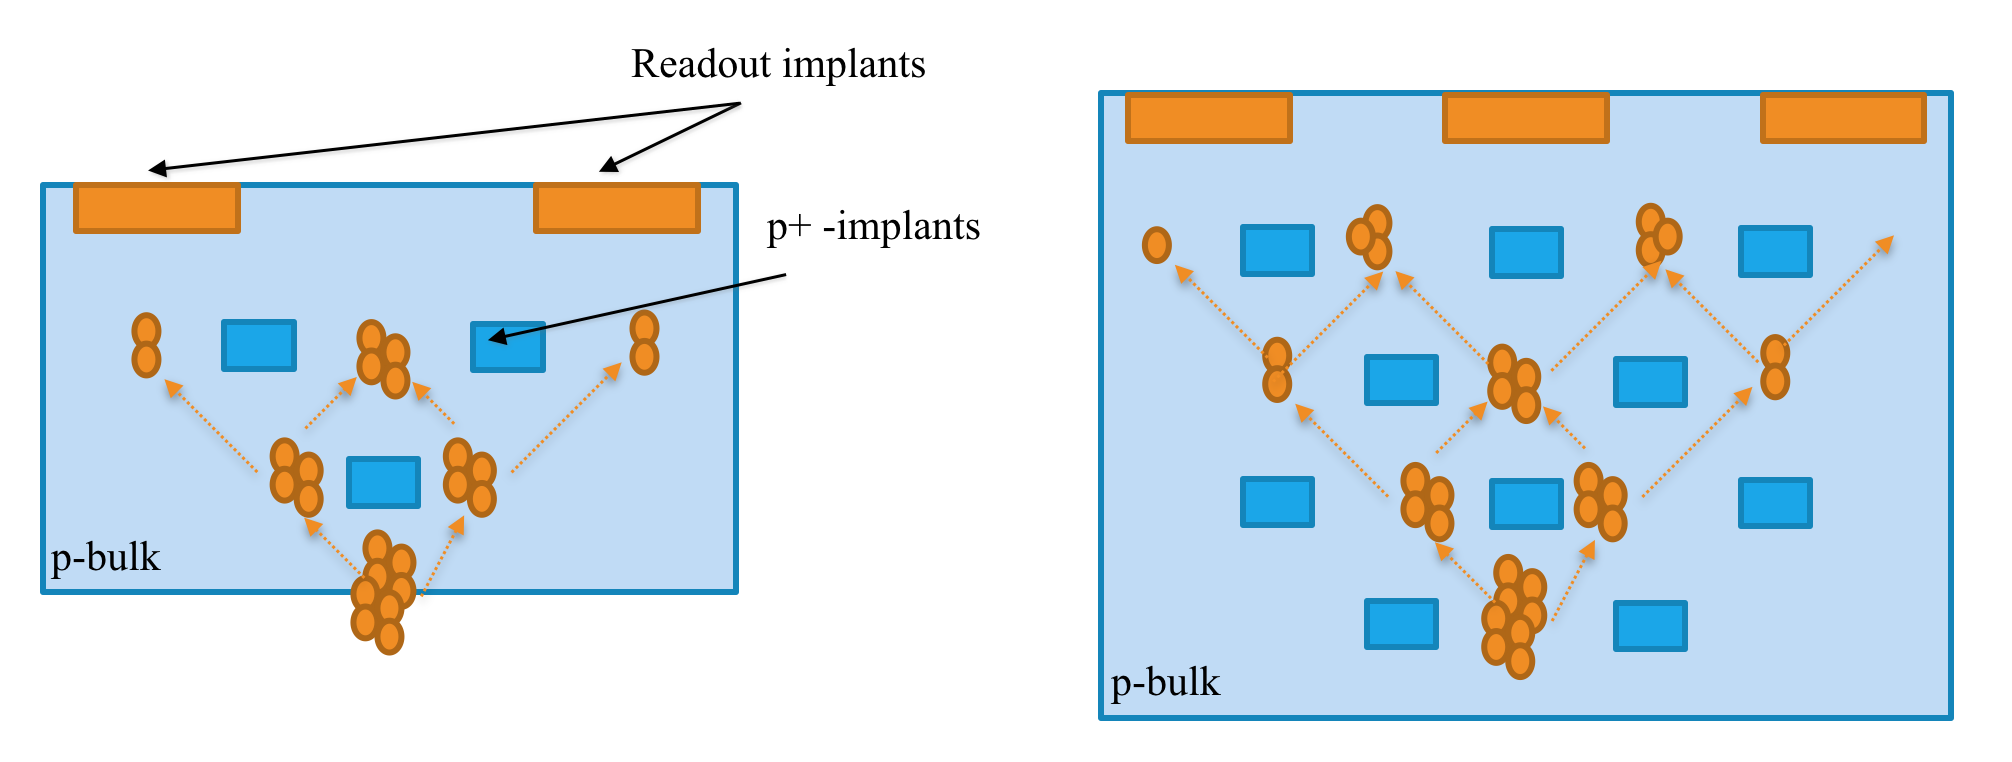
\includegraphics[width=12cm]{/Users/tweety/Documents/PhD/TIPP/TIPP17/pictures/binomial.png}}

Fig. 1. The example of the 50/50 charge sharing in the ELAD sensor. 
\end{figure}

The binomial charge distribution gives a cluster size of 3 that is not optimal. The neighboring strips may collect not enough charge to pass the sensor's threshold. More efficient charge sharing is achieved at a value of cluster size of 2. In order to obtain this value of the cluster size, it is necessary to change the position of the implants. Usage of p+ deep implants leads to the increase of the value of the doping concentration in the sensor. This causes to increasing of the value of $N_{eff}$. The high value of $N_{eff}$ induces the increase of the depletion voltage. 

\begin{equation}
N_{eff}=N_{D}-N_{A}
\end{equation}

\begin{equation}
V_{depl}=\frac{q_0 D^2 |N_{eff}|}{2 \epsilon_r \epsilon_0 }
\end{equation}

To control the value of $N_{eff}$ deep p+ and n+ implants are used. The implants are located between 2 strips/pixels, which gives a cluster size of 2. The n+ implants are placed between two p+ implants. If the doping concentrations of p+ and n+ implants are carefully balanced, the value of $N_{eff}$ and, correspondingly, $V_{depl}$ remains not to high. The number of implant layers should be as small as possible due to the difficult production process. 

\else
 
In the semiconductor sensors a charged particle creates electron-hole pairs which drift under the influence of an electric field to the read-out electrodes. If all charge carriers are collected by a single strip/pixel, the position resolution depends only on the distance between strips/pixels, i.e. on pitch size. If the lateral broadening of the charge is compared with the strip/pixel pitch, the part of the charge may be collected at a neighboring strip/pixel. This effect, called charge sharing, can improve the accuracy of the position resolution. The charge sharing could be achieved by using the magnetic field, by tilting the sensor or increasing the lateral size of the charge distribution during the drift.

The charge carriers drift along the lines of electric field. In order to spread the charge in the lateral direction, the electric field should be modified. To manipulate the electric field, deep implants are used. The p+ implants in a p-bulk sensor are conceived by incorporation of Boron atoms, and  create a repulsive area for electrons. When the electron cloud meets a p+ implant on the drifting way, the former splits into two halves fig.1 (left). Applying it layer-wise gives the charge sharing between three strips/pixels fig.1 (right).  The charge cloud is split 50/50 on every layer, which gives a binomial distribution of the charge.

\begin{figure}[h]
\center{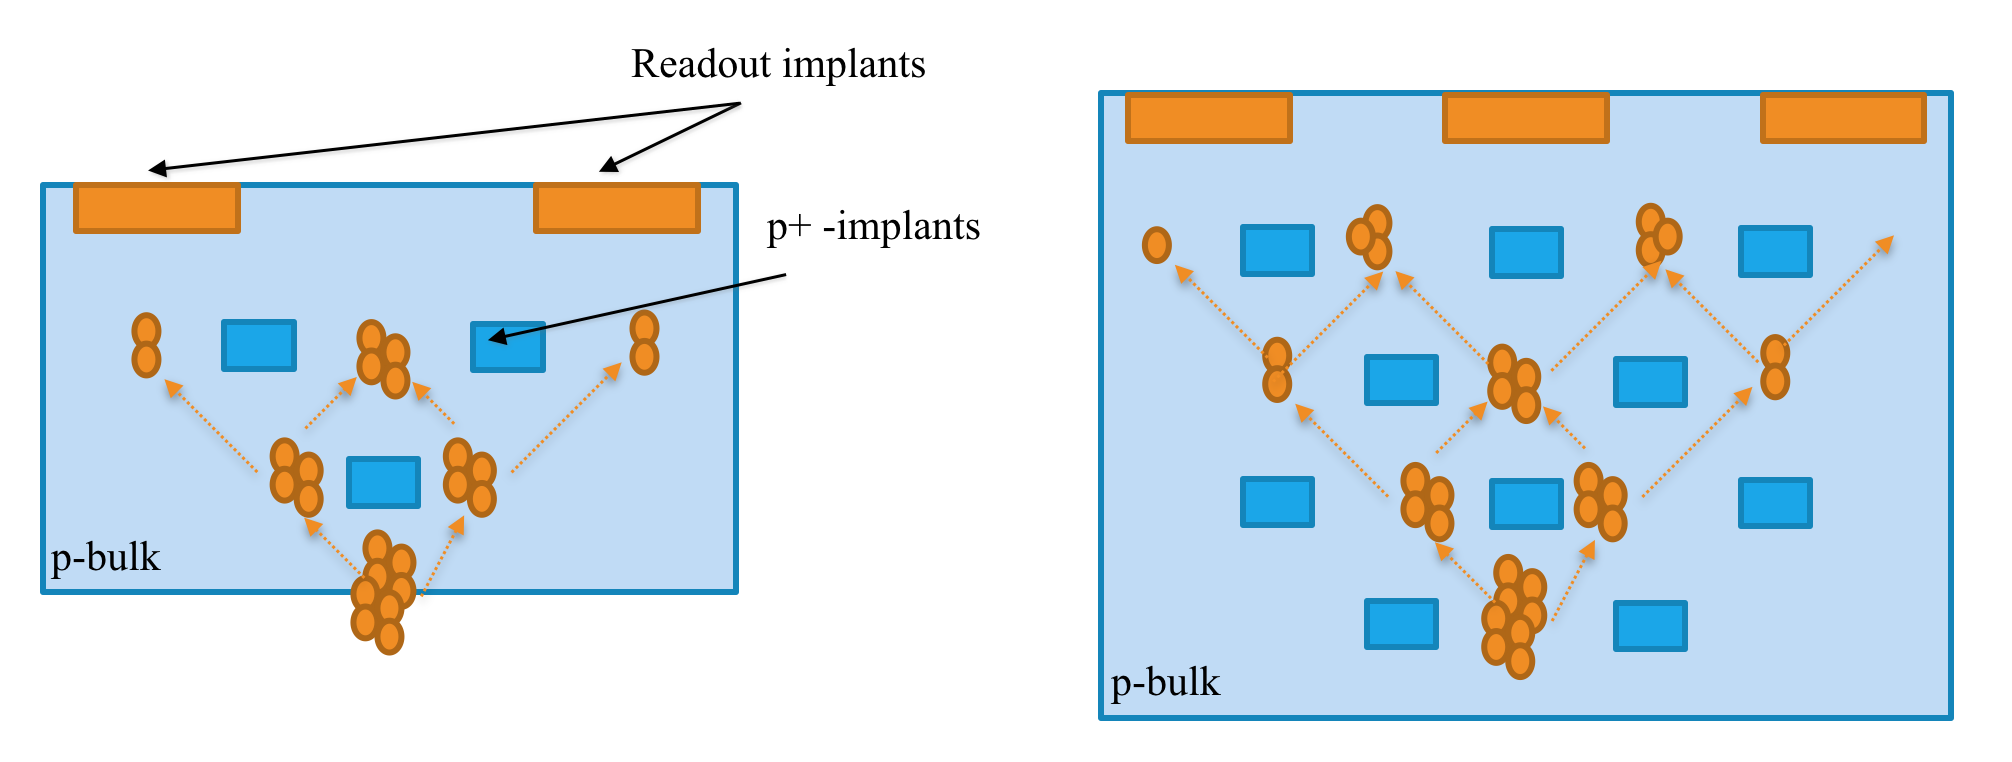
\includegraphics[width=12cm]{/Users/tweety/Documents/PhD/TIPP/TIPP17/pictures/binomial.png}}

Fig. 1. The example of the 50/50 charge sharing in the ELAD sensor. 
\end{figure}

The binomial charge distribution gives a cluster size of 3 that is not optimal. The neighboring strips may collect not enough charge to pass the sensor's threshold. More efficient charge sharing is achieved at a value of cluster size of 2. In order to obtain this value of the cluster size, it is necessary to change the position of the implants. Usage of p+ deep implants leads to the increase of the value of the doping concentration in the sensor. This causes to increasing of the value of $N_{eff}$. The high value of $N_{eff}$ induces the increase of the depletion voltage. 

\begin{equation}
N_{eff}=N_{D}-N_{A}
\end{equation}

\begin{equation}
V_{depl}=\frac{q_0 D^2 |N_{eff}|}{2 \epsilon_r \epsilon_0 }
\end{equation}

To control the value of $N_{eff}$ deep p+ and n+ implants are used. The implants are located between 2 strips/pixels, which gives a cluster size of 2. The n+ implants are placed between two p+ implants. If the doping concentrations of p+ and n+ implants are carefully balanced, the value of $N_{eff}$ and, correspondingly, $V_{depl}$ remains not to high. The number of implant layers should be as small as possible due to the difficult production process. 

\fi

\section{TCAD simulations}
\label{sec:simulations}
\ifdefined\notFOREPJ
% 
Extensive simulation is essential for a new sensor development. 
The  Technology Computer-Aided Design (TCAD) SYNOPSYS was selected  as a tool for simulations, widely used for the development and optimization of semiconductor processing technologies and devices~\cite{Synopsys}. 
In particular, three tools have been exploited: SPROCESS, SDE and SDEVICE. 
%FIXME introduce variable for SPROCESS, SDE, SDEVICE, ...
SPROCESS simulates the fabrication steps in silicon process technologies. 
SDE builds and edits device structures using geometric operations. 
SDEVICE simulates the electrical, thermal, and optical characteristics of silicon and compound semiconductor devices~\cite{SynopsysIncG-2012.06}.

\begin{figure}[t]
\begin{minipage}[h]{0.5\linewidth}
\center{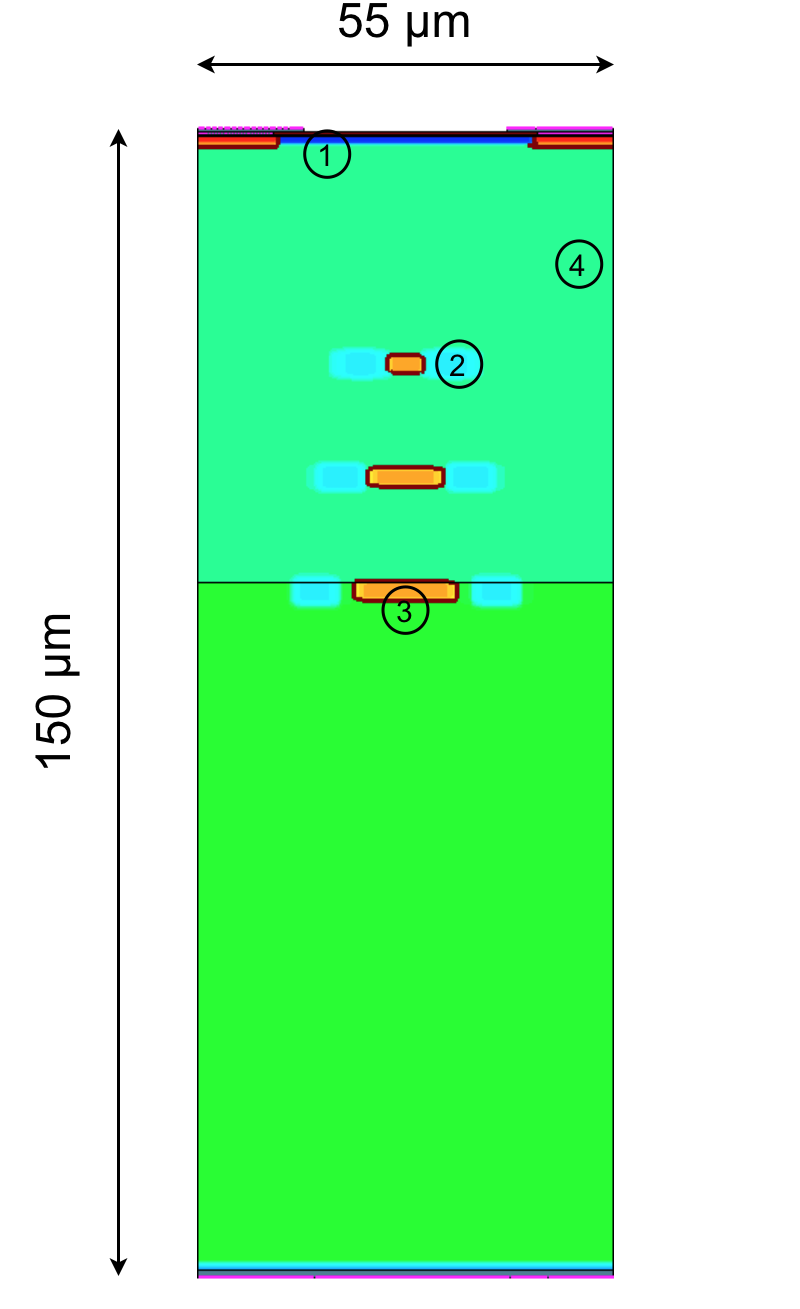
\includegraphics[trim= 0 0 0 0, height=7cm]{pictures/geometry.png} \\ (A)}
\end{minipage}
\hfill 
\begin{minipage}[h]{0.5\linewidth}
\center{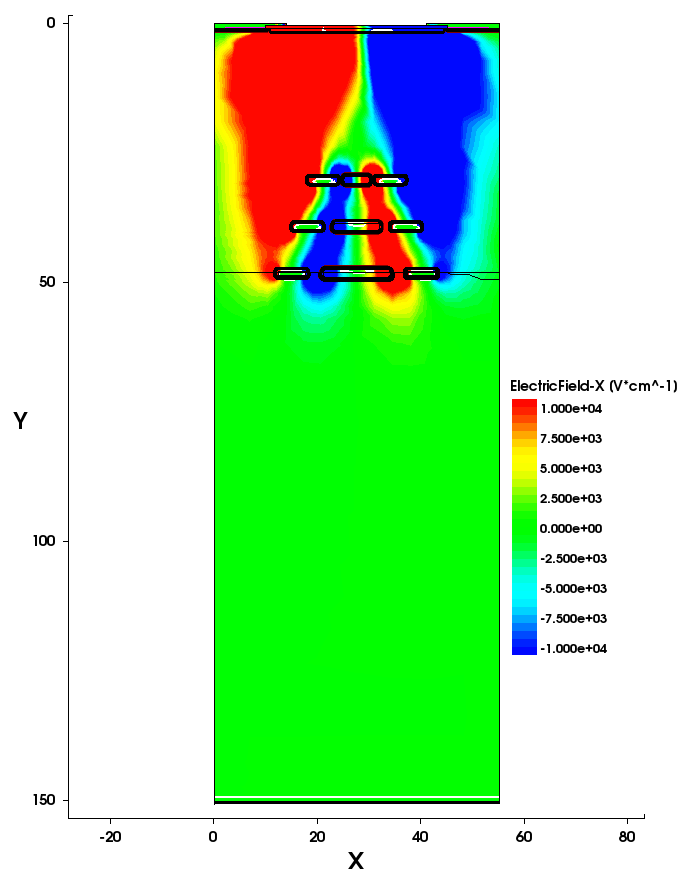
\includegraphics[trim= 0 0 0 0, height=7cm]{pictures/elfield.png} \\(B)}
\end{minipage}
\caption[short description here]
 {(A) TCAD geometry of the ELAD sensor. 1 - p-spray, 2 - deep p-implant, 3 - deep n-implant, 4 - epi-zone. 
 (B) TCAD simulation of the electric field in the ELAD sensor. 
 }
\label{fig:geo-elfield}
\end{figure}

The parameters which should be optimised are the width and depth of implants, distance within/to next layer, position/shift to neighbouring layer,
 the number of layers and optimal doping concentrations for deep implants.
The profile of the electric field yielding an optimal charge sharing is a result of the scan over the mentioned parameters. 

The TCAD geometry of the ELAD sensor Fig. \ref{fig:geo-elfield}~(A) contain p-type sensor, three layers of n and p deep implants, p-spray isolation, readout implants, readout electrodes, SiO${}_2$ and backplane. 
With the p-spray isolation technique a shallow unstructured p implant prevents the build-up of an electron layer below the oxide~\cite{Lutz}. 
The p-spray concentration was chosen according to the value of the breakdown voltage~\cite{Pellegrini}. 
The shape of implants is described by using an error function. 
The total sensor thickness is 150 $\muup$m, the pitch size is 55 $\muup$m in agreement with TimePix3~\cite{TimePix}. readout chip, which is foreseen to be used later on. 

The electric field simulation shows that the p- and n- deep implants lead to changes the potential Fig.~\ref{fig:geo-elfield}~(B). %FIXME lead to cause ?!
The mean electric field is similar to an electric field in a standard design sensor, but the deep implants change the field locally, i.e.\ incuce an electric field component in $x$-direction. %FIXME induce, not include
The charges drift towards the middle between two strips/pixels and change their drift path due to diffusion. %FIXME ... the middle, %FIXME and change their drift path due to diffusion. not clear for the reader
Red zones in Fig.~\ref{fig:geo-elfield}~(B) indicate areas where the electric field force electrons to change their drift path to the right, blue zones - to the left, consequently create the possibility of collecting the charge by two strips. 
%FIXME it is not the read zone that forces any one to do anything, rather: Red zones indicate areas where the eletric field blablabla and therfore electrons drift blablabla. 
In addition the simulation shows that the non-homogeneous electric field in $x$-direction is stable over time. 


\begin{figure}[t]
 \begin{minipage}[h]{0.24\linewidth}
 \center{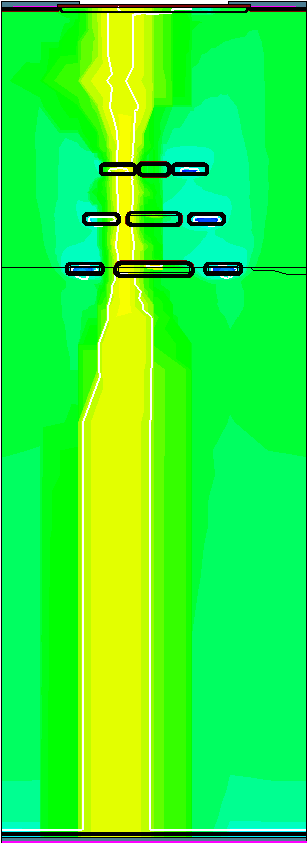
\includegraphics[trim= 0 0 0 0, height=7cm]{pictures/driftt1_1.png} \\ (1)}
 \end{minipage}
 \begin{minipage}[h]{0.24\linewidth}
 \center{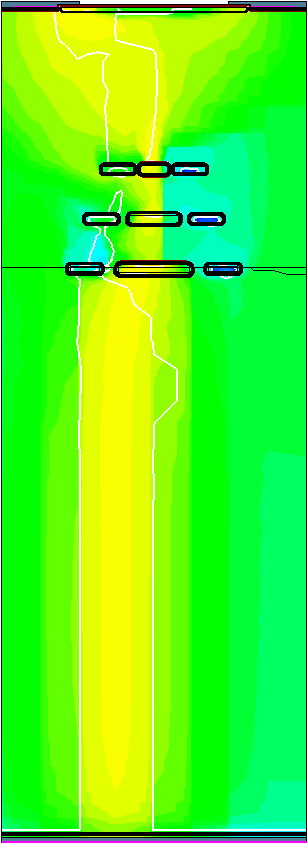
\includegraphics[trim= 0 0 0 0, height=7cm]{pictures/driftt2_1.png} \\(2)}
 \end{minipage}
 \begin{minipage}[h]{0.24\linewidth}
 \center{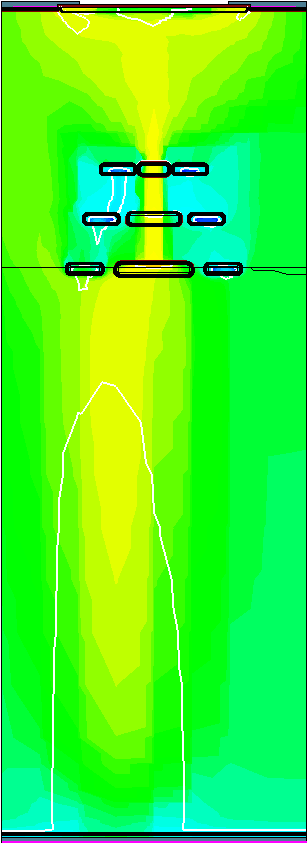
\includegraphics[trim= 0 0 0 0, height=7cm]{pictures/driftt3_1.png} \\(3)}
 \end{minipage}
 \begin{minipage}[h]{0.24\linewidth}
 \center{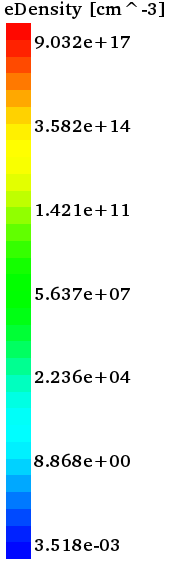
\includegraphics[trim= 0 0 0 0, width=2cm]{pictures/driftscale1.png}}
 \end{minipage}
\caption[short description here]
  {TCAD drift simulation in the ELAD sensor. (1) at $t = \SI{e-12}{\sec}$, (2) at $t = \SI{e-10}{\s}$, (3) at $t = \SI{1.2e-9}{\s}$.}
\label{fig:drift}
\end{figure} %FIXME pictures are of bas quality, use high resolution! or at best vector grpahics (eps file)

To understand the behaviour of charge carriers in the ELAD sensor the drift simulation has been carried out. 
It shows that the charge carriers created near an electrode are collected by it, but the charge created beneath the deep implants area %FIXME It shows (GRAMMAR: because the simluations still show that, they have not stopped showing that)
 changes its drift path and is collected by two strips Fig.~\ref{fig:drift}.  
Thereby, the drift simulation supports the basic concept of charge sharing in ELAD sensors making use of a non-homogeneous electric field in $x$-direction. 


 
\else
 
Extensive simulation is essential for a new sensor development. 
The  Technology Computer-Aided Design (TCAD) SYNOPSYS was selected  as a tool for simulations, widely used for the development and optimization of semiconductor processing technologies and devices~\cite{Synopsys}. 
In particular, three tools have been exploited: SPROCESS, SDE and SDEVICE. 
%FIXME introduce variable for SPROCESS, SDE, SDEVICE, ...
SPROCESS simulates the fabrication steps in silicon process technologies. 
SDE builds and edits device structures using geometric operations. 
SDEVICE simulates the electrical, thermal, and optical characteristics of silicon and compound semiconductor devices~\cite{SynopsysIncG-2012.06}.

\begin{figure}[t]
\begin{minipage}[h]{0.5\linewidth}
\center{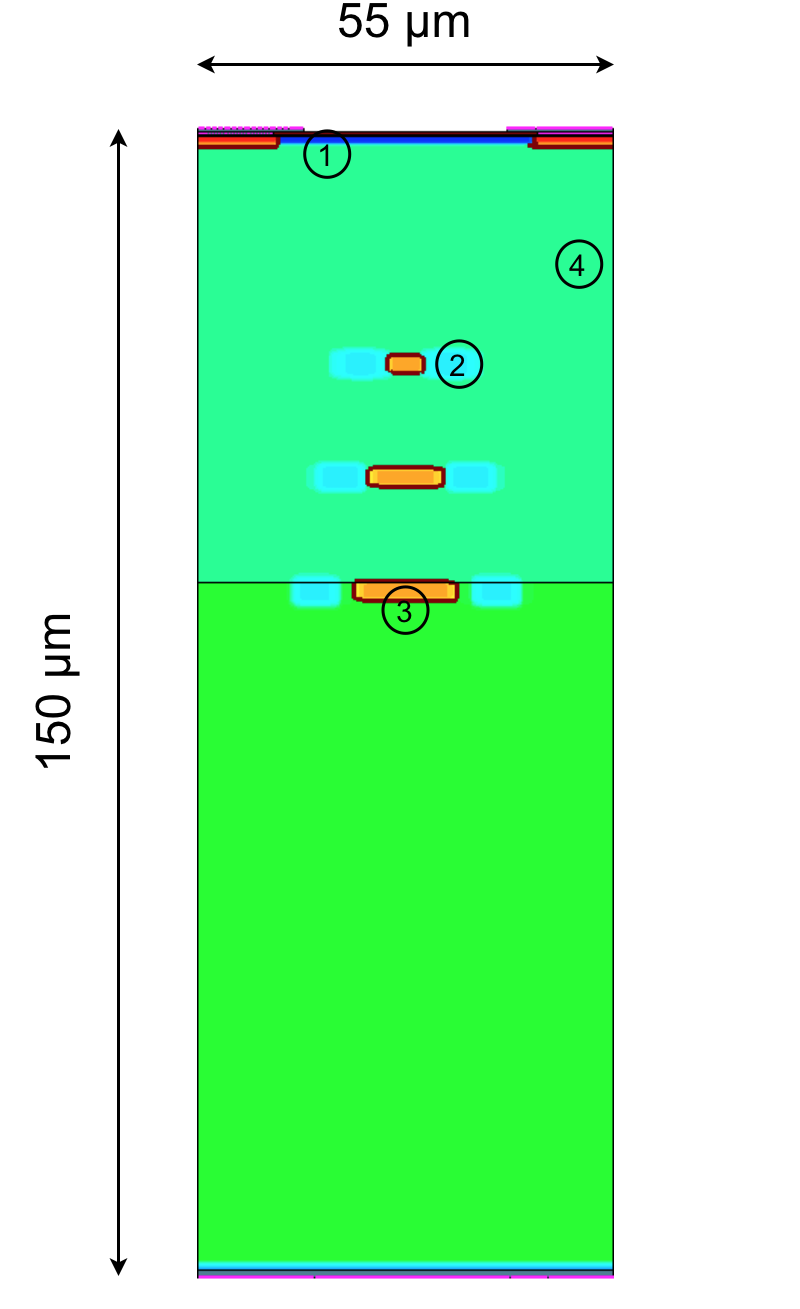
\includegraphics[trim= 0 0 0 0, height=7cm]{pictures/geometry.png} \\ (A)}
\end{minipage}
\hfill 
\begin{minipage}[h]{0.5\linewidth}
\center{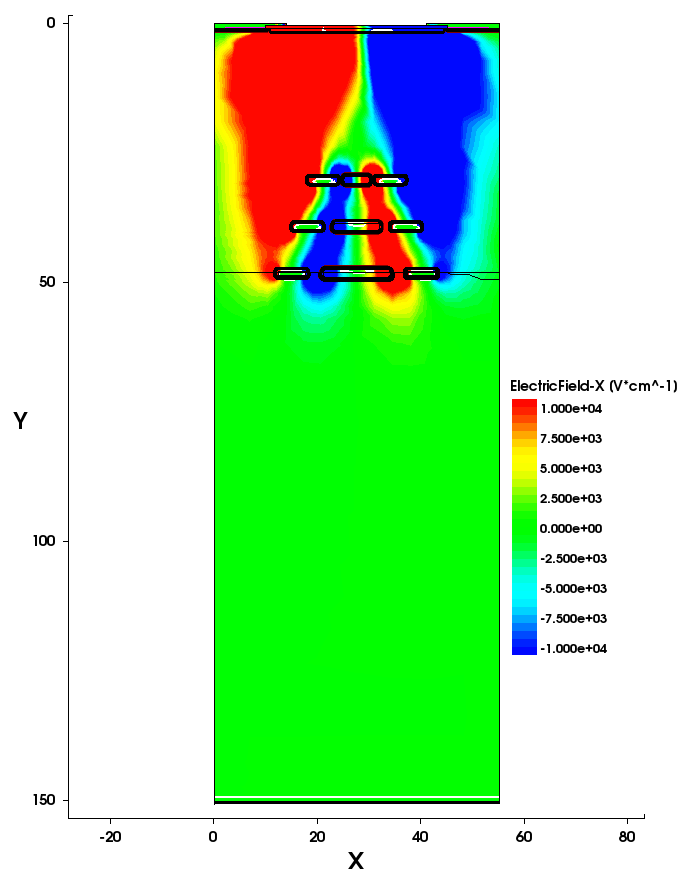
\includegraphics[trim= 0 0 0 0, height=7cm]{pictures/elfield.png} \\(B)}
\end{minipage}
\caption[short description here]
 {(A) TCAD geometry of the ELAD sensor. 1 - p-spray, 2 - deep p-implant, 3 - deep n-implant, 4 - epi-zone. 
 (B) TCAD simulation of the electric field in the ELAD sensor. 
 }
\label{fig:geo-elfield}
\end{figure}

The parameters which should be optimised are the width and depth of implants, distance within/to next layer, position/shift to neighbouring layer,
 the number of layers and optimal doping concentrations for deep implants.
The profile of the electric field yielding an optimal charge sharing is a result of the scan over the mentioned parameters. 

The TCAD geometry of the ELAD sensor Fig. \ref{fig:geo-elfield}~(A) contain p-type sensor, three layers of n and p deep implants, p-spray isolation, readout implants, readout electrodes, SiO${}_2$ and backplane. 
With the p-spray isolation technique a shallow unstructured p implant prevents the build-up of an electron layer below the oxide~\cite{Lutz}. 
The p-spray concentration was chosen according to the value of the breakdown voltage~\cite{Pellegrini}. 
The shape of implants is described by using an error function. 
The total sensor thickness is 150 $\muup$m, the pitch size is 55 $\muup$m in agreement with TimePix3~\cite{TimePix}. readout chip, which is foreseen to be used later on. 

The electric field simulation shows that the p- and n- deep implants lead to changes the potential Fig.~\ref{fig:geo-elfield}~(B). %FIXME lead to cause ?!
The mean electric field is similar to an electric field in a standard design sensor, but the deep implants change the field locally, i.e.\ incuce an electric field component in $x$-direction. %FIXME induce, not include
The charges drift towards the middle between two strips/pixels and change their drift path due to diffusion. %FIXME ... the middle, %FIXME and change their drift path due to diffusion. not clear for the reader
Red zones in Fig.~\ref{fig:geo-elfield}~(B) indicate areas where the electric field force electrons to change their drift path to the right, blue zones - to the left, consequently create the possibility of collecting the charge by two strips. 
%FIXME it is not the read zone that forces any one to do anything, rather: Red zones indicate areas where the eletric field blablabla and therfore electrons drift blablabla. 
In addition the simulation shows that the non-homogeneous electric field in $x$-direction is stable over time. 


\begin{figure}[t]
 \begin{minipage}[h]{0.24\linewidth}
 \center{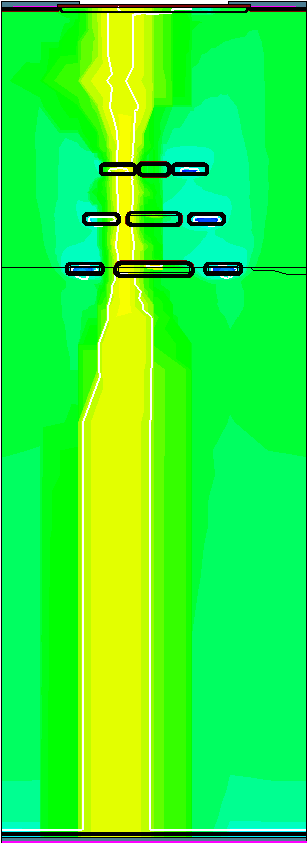
\includegraphics[trim= 0 0 0 0, height=7cm]{pictures/driftt1_1.png} \\ (1)}
 \end{minipage}
 \begin{minipage}[h]{0.24\linewidth}
 \center{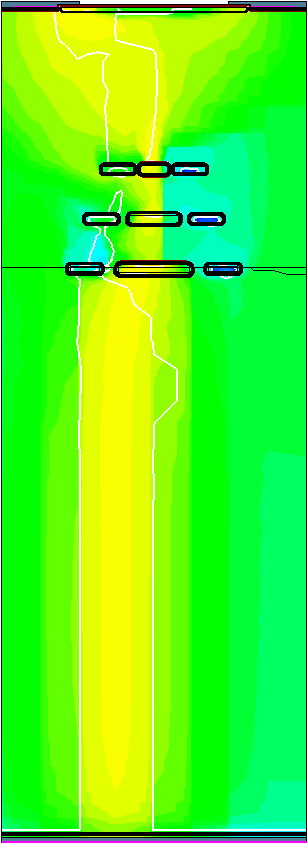
\includegraphics[trim= 0 0 0 0, height=7cm]{pictures/driftt2_1.png} \\(2)}
 \end{minipage}
 \begin{minipage}[h]{0.24\linewidth}
 \center{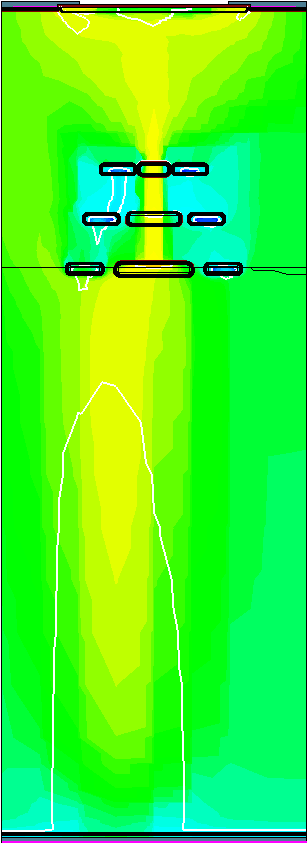
\includegraphics[trim= 0 0 0 0, height=7cm]{pictures/driftt3_1.png} \\(3)}
 \end{minipage}
 \begin{minipage}[h]{0.24\linewidth}
 \center{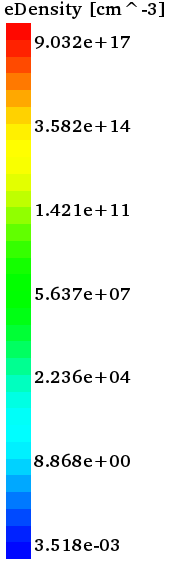
\includegraphics[trim= 0 0 0 0, width=2cm]{pictures/driftscale1.png}}
 \end{minipage}
\caption[short description here]
  {TCAD drift simulation in the ELAD sensor. (1) at $t = \SI{e-12}{\sec}$, (2) at $t = \SI{e-10}{\s}$, (3) at $t = \SI{1.2e-9}{\s}$.}
\label{fig:drift}
\end{figure} %FIXME pictures are of bas quality, use high resolution! or at best vector grpahics (eps file)

To understand the behaviour of charge carriers in the ELAD sensor the drift simulation has been carried out. 
It shows that the charge carriers created near an electrode are collected by it, but the charge created beneath the deep implants area %FIXME It shows (GRAMMAR: because the simluations still show that, they have not stopped showing that)
 changes its drift path and is collected by two strips Fig.~\ref{fig:drift}.  
Thereby, the drift simulation supports the basic concept of charge sharing in ELAD sensors making use of a non-homogeneous electric field in $x$-direction. 


 
\fi


\section{Production}
\label{sec:discussion}
\ifdefined\notFOREPJ
% For ELAD sensor production is necessary to create a new manufacture technology. This new technology involve surface implantation and epitaxial growing. Epitaxial growing means growing of the crystal in the correct lattice structure on top of a single-crystal wafer [3]. One of the methods of epitaxial growing is a CVD method. Chemical Vapor Deposition (CVD) is the deposition of a solid material onto a heated substrate through a chemical reaction of compounds contained the gas passing over the substrate. The temperature in CVD method is around $1100^\circ C$. The surface implantation implemented by bombarding the substrate with accelerated ions.

The ELAD production includes several steps. First, on a p-type wafer, the first layer of deep implants is generated by surface implantation. Then, on the implanted wafer creates an epitaxial layer, in the surface of this epitaxial zone, puts the second layer of deep implants and the process repeats. 

The dangerous side of such production is a possibility of implants to diffuse during the CVD process, but TCAD process simulation shows that the difference in sizes of deep implants before and after 20 min heating up to $1100^\circ C$ less than 1 $\mu m$.
\else
 For ELAD sensor production is necessary to create a new manufacture technology. This new technology involve surface implantation and epitaxial growing. Epitaxial growing means growing of the crystal in the correct lattice structure on top of a single-crystal wafer [3]. One of the methods of epitaxial growing is a CVD method. Chemical Vapor Deposition (CVD) is the deposition of a solid material onto a heated substrate through a chemical reaction of compounds contained the gas passing over the substrate. The temperature in CVD method is around $1100^\circ C$. The surface implantation implemented by bombarding the substrate with accelerated ions.

The ELAD production includes several steps. First, on a p-type wafer, the first layer of deep implants is generated by surface implantation. Then, on the implanted wafer creates an epitaxial layer, in the surface of this epitaxial zone, puts the second layer of deep implants and the process repeats. 

The dangerous side of such production is a possibility of implants to diffuse during the CVD process, but TCAD process simulation shows that the difference in sizes of deep implants before and after 20 min heating up to $1100^\circ C$ less than 1 $\mu m$.
\fi


\section{Conclusion}
\label{sec:conclusion}
\ifdefined\notFOREPJ
 %
The ELAD sensor it's a new sensor concept that allows for the possibility to achieve an improved position resolution with no need of making a smaller pitch or increasing the number of readout channels. 
The resolution improvement in ELAD sensors is accomplished by increasing the lateral size of the charge distribution. 
For this purpose, deep implants are included in the ELAD sensors. 
The characteristic length, which affects the spatial resolution is the distance between the deep implants rather than the pitch size. 
Dedicated simulations, conducted in the TCAD framework, prove that the charge sharing in ELAD sensors is possible. 
A new plan for a production technique for multi-layered structures with implantation was discussed. 

\else
 
The ELAD sensor it's a new sensor concept that allows for the possibility to achieve an improved position resolution with no need of making a smaller pitch or increasing the number of readout channels. 
The resolution improvement in ELAD sensors is accomplished by increasing the lateral size of the charge distribution. 
For this purpose, deep implants are included in the ELAD sensors. 
The characteristic length, which affects the spatial resolution is the distance between the deep implants rather than the pitch size. 
Dedicated simulations, conducted in the TCAD framework, prove that the charge sharing in ELAD sensors is possible. 
A new plan for a production technique for multi-layered structures with implantation was discussed. 

\fi

%\ifdefined\notFOREPJ
%\else
\section*{Acknowledgements}

{\small
\section*{Data and materials}
%The datasets supporting the conclusions of this article are available from reference \cite{jansen_data}.
%The software used is available from the github repositories: 1) \url{https://github.com/eutelescope/eutelescope}, 2) \url{https://github.com/simonspa/eutelescope/}, branch \textit{scattering}
% and 3) \url{https://github.com/simonspa/resolution-simulator}.
%For the presented analysis, these specific tags have been used: \cite{jansen_2016_49065}.

% \section*{Competing interests}
% The authors declare that they have no competing interests.


\bibliographystyle{IEEEtran}
\ifdefined\notFOREPJ
\bibliography{bibtex/refs}
\else
\bibliography{refs}
\fi
}

\end{document}


\grid
